\documentclass{jtacs}
\usepackage{placeins}

\begin{document}
\title{A study on the effectiveness of investment strategy based on the concept of pivot points levels using  Matthews criterion}
\markboth{A. Wilinski, T. Nyczaj, A. Bera, P. Blaszynski}{}
\maketitle

\xauthor{Antoni Wilinski$^1$, Tomasz Nyczaj$^1$, Aneta Bera$^1$, Piotr Blaszynski$^{1}$}
\xaffiliation{$^1$ Faculty of Computer Science and Information Technology, West Pomeranian University of Technology, Szczecin, Poland}
\xemail{\{awilinski, tnyczaj, abera, pblaszynski\}@wi.zut.edu.pl}

\begin{abstract}%
In this work, the possibility of assessing traditional investment strategy based on the pivot points for using with other than the commonly used criterion is examined. The authors attempted to apply the Matthews Correlation Coefficient (further reffered as MCC)  criterion based on a confusion matrix when assessing the strategy to include more factors than the traditional criteria (such as profit, profit vs. Risk, Sharpe ratio, Calmar ratio) and to express these factors by one number. The criterion based on a confusion matrix is, in authors beliefs, unique in this application and gives a fairly valuable estimation of trading strategy. An example of several strategies tested on EURUSD 1h time series in selected intervals in the years 2012-2013 is considered. Among these strategies there is a simple strategy based on the concept of pivot points levels and more complex derivative strategies, based on the vector of optimized values of certain parameters. These strategies are evaluated using both traditional criteria and modification of MCC proposed by the authors. 
\end{abstract}

\begin{keywords}%
algorithmic trading, machine learning, investment strategies, confusion matrix%
\end{keywords}

%
\section{Introduction}
Confusion matrix is a well-known criterion for assessing the quality of classification in machine learning, however, it does not give a clear answer which classifier is better\cite{provost} \cite{lewis} \cite{burke}. On its basis a number of additional measures of classification quality \cite{hay}, such as accuracy, precision, sensitivity, specificity, etc \cite{baldi} are built. One of additional measures derived from the confusion matrix is the Matthews criterion \cite{matthews}. It is so much more convenient than the original confusion matrix that is a number, not a matrix. Authors realize, however, that such a measure of the quality of the classification also has its drawbacks (like all the criteria or their sets used to evaluate the quality of investment strategies - Sharpe ratio, Calmar ratio or set of indicators). \\

	In the analysis of the confusion matrix a False Positive error that is a Type I error and the False Negative error that is a Type II error (Type II error \cite{burke}) are defined. If one considers the hypothesis that the test subject has cancer or that the observed passenger is a terrorist, a type I error causes less impact than the type II error (in common sense it is better to err in thinking that someone has cancer, than being wrong and believing that the patient is healthy; it is better to make a mistake by assessing that the observed passenger is a terrorist, than not recognizing one, when in fact he/she is). When considering the hypothesis that is needed to open long positions, because under certain conditions of close it will bring profit - type I error is more painful for the investor (as he/she lose) than type II error (no open positions). Therefore, you can define the following correct decisions and mistakes made by the investor, eg during strategy testing of open long positions only:
\begin{itemize}
\item True  Positive (TP) –-- when the investor believes that the market price of the observed asset will increase, and in fact it happens;
\item False Positive (FP)  --– when the investor believes that the market price will increase and in reality the price drops;
\item True Negative (TN) --– when the investor believes that the observed price will drop and does not open a position, and in fact he is right;
\item False Negative (FN) --– when the investor believes that the observed price will drop and does not open a position, while in reality, the price rose and a chance for another profit was lost.
\end{itemize}
A similar analysis can be performed for the cases of other strategy that opens only short positions - with reversed conclusions.\\
Taking into account the above definitions, Matthews has already developed several years ago a formula, in which the matrix of all the events and decisions is summed up using  MCC indicator:
\begin{equation}
MCC = \frac{TP \cdot TN - FP \cdot FN}{(TP+FP)(TP+FN)(TN+FP)(TN+FN)}
\end{equation}
In this index all the possible successes and failures as well as their frequency are taken into account simultaneously. In addition, this index is a number in the range $[-1, 1]$ giving a view of the inverse of the total predictability ($-1$), full of randomness ($0$) or full predictability of events ($1$).\\
Other quality prediction indicators, described below, such as Sharpe ratio or Calmar ratio have obvious drawbacks and thus many practitioners of investment process use multi-criteria evaluation method to find the effectiveness of the strategy. Such sets of indicators are referred in a popular investment platform Metatrader \cite{wang} and include, among others, factors such as average profit, the average loss, the number of consecutive successes and failures, the largest drawdown,  the number of successes to the number of failures, etc. Profit for long positions is calculated as difference between price of buy and price of sell including spread, similarly for short positions this is difference between sell and buy price with a negative sign. The loss on the position is when the profit is less than zero.\\
The authors of this publication referring to the market practice consider Calmar \cite{sinclare} as a very good synthetic indicator, which unfortunately also has an apparent drawback - with very long investment horizon it overstates investors optimistic who starts using a particular strategy.\\
The authors believe that the MCC indicator does not have this disadvantage. Regardless of the size of the time window in which a certain strategy would be considered and a MCC indicator would be applied there, it should give similar value (for a given strategy), as long as the strategy takes into account all the possible trends. The strategy considered here meets this challenge. Figure \ref{rys1} shows a fragment of the time series for EURUSD 1h showing both the downward trend, rising trend and fragments, which can be considered as cycles or horizontal trend. EURUSD is most popular currency pairs and has smallest spread value. One hour interval matches the frequency of the transaction and this pair has sufficient volatility at said interval to consider it for the algorithmic trading purposes. 
\begin{figure}[ht]
\centering
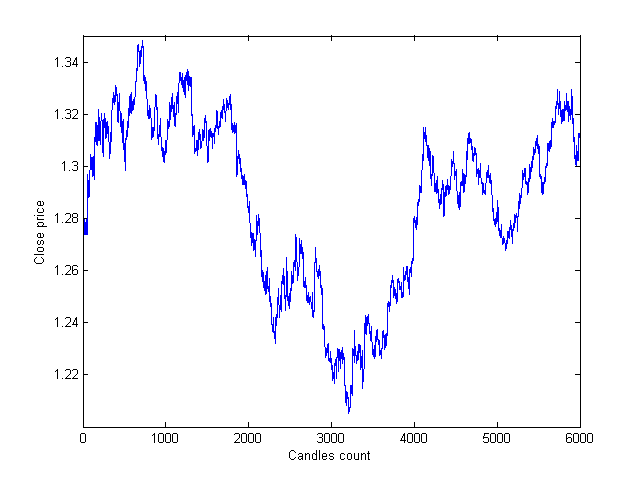
\includegraphics[width = 0.6\textwidth]{pictures/researched_data.png}
\caption{A fragment of the time series EURUSD 1h on which strategy was tested}
\label{rys1}
\end{figure}
\FloatBarrier

% % % % % % % % % % % % % % % % % % % % % % % % % %
\section{Research of the simple strategy based on pivot points}
Pivot points (further referred to as PP) are certain contractual levels considered in the candle (or in few further candles), calculated on the basis of data from the past. According to popular sources \cite{person} \cite{myers} there are many ways (algorithms) to calculate Pivot levels. The authors treat these formulas as suggestions (treated as an inspiration rather than as dogmas). It can be easily demonstrated, that strategies based on the idea of pivot points in the original form have low effectiveness. This low efficiency is demonstrated in the article. At the same time, the authors of this study demonstrate higher effectiveness of the strategies based on more complex investment algorithms coming from the same concept of Pivot levels.\\

The first strategy that the authors consider in this paper is a strategy, as simple as possible, based directly on the pivot points formulas that are suggested in many sources  \cite{person}\cite{myers}\cite{tian}. The second strategy is an extension of the first one, with several parameters, that are optimized in machine learning, added.\\

In the first approach, the PP is treated as a simple, consistent and repeatable operation. After the end of the next candle, pivot points \cite{person} and all derivative levels are calculated using traditional (optionally modified) formulas, and then immediately, depending on the situation, long or short positions are opened. This position is closed at the end of the candle in which it was opened.\\

The first simple type of strategy is as follows. \\
Usually there are 4 (rarely 6) defined pivot points levels \cite{person} \cite{myers}. The top two are called resistance levels (R1, R2), bottom two - support levels (S1, S2). There are different formulas, but the most popular \cite{person} are:
\begin{equation}
P= \frac{(H+L+C)}{3}
\end{equation}
\begin{equation}
R1=2 \cdot P-L
\end{equation}
\begin{equation}
S1=2 \cdot P-H
\end{equation}
\begin{equation}
R2=P+(R1-S1)
\end{equation}
\begin{equation}
S2=P-(R1-S1)
\end{equation}
For the portion of the surveyed data, curves described using aforementioned formulas may look like the ones in the Figure \ref{rys2}.
\begin{figure}[ht]
\centering
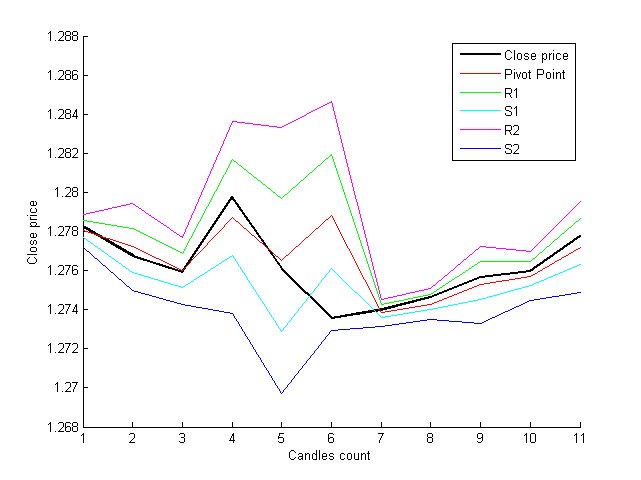
\includegraphics[width = 0.6\textwidth]{pictures/samplePP2.png}
\caption{Relative position of the PP levels and levels of resistance and support}
\label{rys2}
\end{figure}
\FloatBarrier
The graph shows how the level of PP oscillates between the respective levels of support and resistance and how periodically intersects them.\\

The strategy relies on stating four different hypotheses about the further course prices, depending on where the closing price is on the ,,scale'' levels calculated at the close of the candle. This is authored strategy, although not very original. In the literature one can find a lot of suggestions to behave that way \cite{murphy}\cite{krutsinger}\cite{elder}. Of course, there are also other possible hypotheses and strategies based on them \cite{wilinskir}.\\

Therefore, it is believed, that if the price upward or downward deviation on the opening of the following candle is considered very high (above R2 or below S2), one has to deal with the trend (increasing or declining) and should open position to the ,,outside''. If the price is located between levels R1 and R2, or S1 and S2, it should be presumed that the trend is horizontal and one has to open position to  the inside. If the price is quite neutral, between S1 and R1, no action is necessary.\\

Presented classification allows to define four decision situations --- four sub strategies, hereafter referred to as A ... D.
\begin{itemize}
\item A - Sub strategy triggered when current price deviates upward above the R2 level. Then investor (or machine) will open long position. Position will be closed at the close of the current candle --- after one candle interval. Similarly in next sub strategies.
\item B - Sub strategy triggered when current price is above R1 level and at the same time above R2 level. Then investor will open short position.
\item C - Sub strategy triggered when current price is above S2 level and at the same time below S1 level. Then investor will open long position.
\item D - Sub strategy triggered when current price is below S2 level. Then investor will open short position.
\end{itemize}
It is worth noting that due to the uncertainty, when the price is close to the PP, no position will be opened if the price is inside the band between S1 and R1 level. This simplest strategy gives the following results for the considered data set. \\

For sub strategy A, Figure \ref{rys3} presents how cumulative profit has changed during tested candles. 
\begin{figure}[ht]
\centering
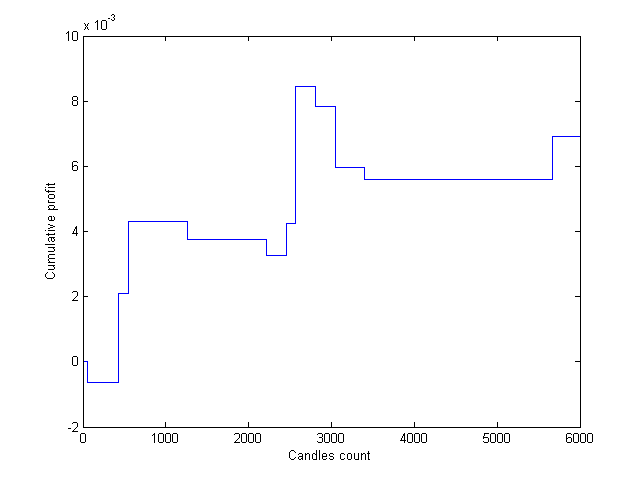
\includegraphics[width = 0.5\textwidth]{pictures/PivotPointsAp.png}
\caption{Cumulative profit for simple sub strategy A}
\label{rys3}
\end{figure}
\FloatBarrier

For this strategy confusion matrix is is presented in Table \ref{tab1}
\begin{table}[ht]
\centering
\caption{Confusion matrix for simple sub strategy A}
\label{tab1}
\begin{tabular}{|l|l|l|}\hline
&	Actual = profit	& Actual = loss\\ \hline
Prediction = profit & $5$	& $6$ \\ \hline
Prediction = loss &	$2409$ &	$3579$ \\ \hline
\end{tabular}
\end{table}
\FloatBarrier
\noindent and Matthews correlation coefficient is $MCC=0.0046$.\\
\noindent The final results for this simple strategy A:
\begin{itemize}
\item Profit: $0.0069$
\item Calmar: $2.432$
\end{itemize}
Analyzing the course chart it can be seen that there are: a small number of opened positions, balance in the number of wins and losses, and the final profit. \\

Subsequently, studies were carried out for the next of these four strategies - simple sub strategy B. Confusion matrix - as presented below - was obtained by an even smaller number of events (only 5). For this strategy confusion matrix is as presented in Table \ref{tab2}
\begin{table}[ht]
\centering
\caption{Confusion matrix for simple sub strategy B}
\label{tab2}
\begin{tabular}{|l|l|l|}\hline
&	Actual = profit	& Actual = loss\\ \hline
Prediction = profit & $4$	& $1$ \\ \hline
Prediction = loss &	$2397$ &	$3597$ \\ \hline
\end{tabular}
\end{table}
\FloatBarrier
\noindent and Matthews correlation coefficient is $MCC=0.0236$.\\
Cumulative return curve is presented in the Figure \ref{rys4}.
\begin{figure}[ht]
\centering
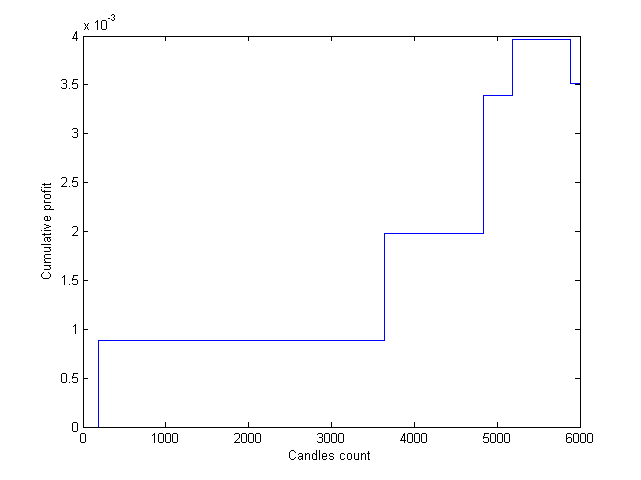
\includegraphics[width = 0.5\textwidth]{pictures/PivotPointsBp.png}
\caption{Cumulative profit for simple sub strategy B}
\label{rys4}
\end{figure}
\FloatBarrier
\noindent Final result for sub strategy B:
\begin{itemize}
\item Profit: $0.0035$
\item Calmar: $7.80$
\end{itemize}
The value of Calmar ratio is impressive, but given that the number of items is small it is rather coincidence and can be treated just as an interesting fact.\\

Next studies were carried out for a simple sub strategy C which gave confusion matrix as in Table \ref{tab3}
\begin{table}[ht]
\centering
\caption{Confusion matrix for simple sub strategy C}
\label{tab3}
\begin{tabular}{|l|l|l|}\hline
&	Actual = profit	& Actual = loss\\ \hline
Prediction = profit & $9$	& $1$ \\ \hline
Prediction = loss &	$2405$ &	$3584$ \\ \hline
\end{tabular}
\end{table}
\FloatBarrier
\noindent and Matthews correlation coefficient is $MCC=0.0415$.\\
Cumulative return curve is presented in the Figure \ref{rys5}.
\begin{figure}[ht]
\centering
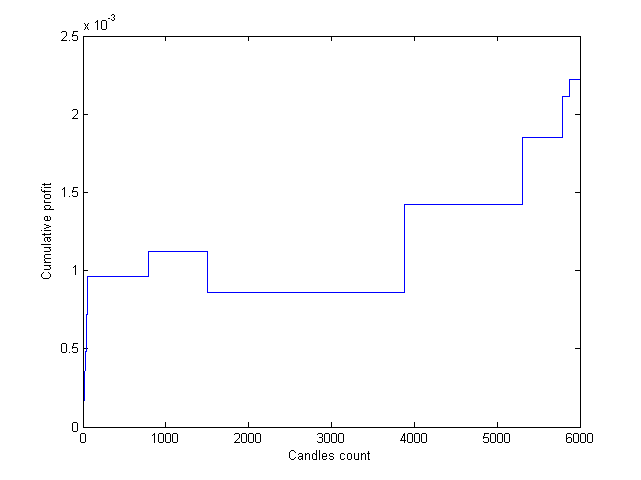
\includegraphics[width = 0.5\textwidth]{pictures/PivotPointsCp.png}
\caption{Cumulative profit for simple sub strategy C}
\label{rys5}
\end{figure}
\FloatBarrier
\noindent Final result for sub strategy C:
\begin{itemize}
\item Profit: $0.0022$
\item Calmar: $8.539$
\end{itemize}

Last tested strategy was sub strategy D. Obtained confusion matrix is presented in Table \ref{tab4}
\begin{table}[ht]
\centering
\caption{Confusion matrix for simple sub strategy D}
\label{tab4}
\begin{tabular}{|l|l|l|}\hline
&	Actual = profit	& Actual = loss\\ \hline
Prediction = profit & $1$	& $13$ \\ \hline
Prediction = loss &	$2400$ &	$3585$ \\ \hline
\end{tabular}
\end{table}
\FloatBarrier
\noindent and Matthews correlation coefficient is $MCC=-0.0325$.\\
Cumulative return curve is presented in the Figure \ref{rys6}.
\begin{figure}[ht]
\centering
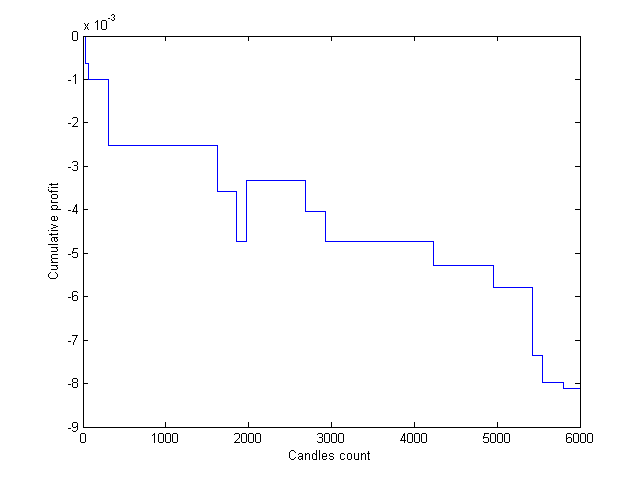
\includegraphics[width = 0.5\textwidth]{pictures/PivotPointsDp.png}
\caption{Cumulative profit for simple sub strategy D}
\label{rys6}
\end{figure}
\FloatBarrier
\noindent Final result for sub strategy D:
\begin{itemize}
\item Profit: $-0.0081$
\item Calmar: $-1.00$
\end{itemize}

This is the only of the four strategies ending with loss, also with a small number of openings and not reliable end result.\\

Much more interesting conclusion may be a summary of all four sub strategies. After all, they can be run simultaneously, under the conditions provided in the PP. After adding all the results accumulated profit curve can be presented as in Figure \ref{rys7}. Obtained confusion matrix is presented in Table \ref{tab5}
\begin{table}[ht]
\centering
\caption{Confusion matrix for summary of all simple sub strategies}
\label{tab5}
\begin{tabular}{|l|l|l|}\hline
&	Actual = profit	& Actual = loss\\ \hline
Prediction = profit & $19$	& $21$ \\ \hline
Prediction = loss &	$9611$ &	$14345$ \\ \hline
\end{tabular}
\end{table}
\FloatBarrier
\noindent and Matthews correlation coefficient is $MCC=0.0061$.
\begin{figure}[ht]
\centering
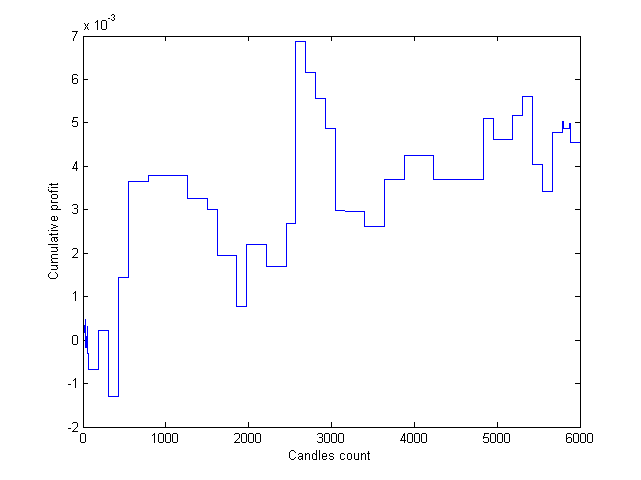
\includegraphics[width = 0.5\textwidth]{pictures/PivotPointsSp.png}
\caption{Cumulative profit for simple strategy S}
\label{rys7}
\end{figure}
\FloatBarrier
\noindent Final result:
\begin{itemize}
\item Profit: $0.0045$
\item Calmar: $1.07$
\end{itemize}

In this ,,generalized'' strategy $40$ positions have been opened. However, the result is not very exciting. This confirms authors suppositions, that this simple strategy, despite incentives from many practitioners, is inefficient and fraught with huge risk.\\

Sub strategy A gave a positive final result with a profit higher than the profit from all four sub strategies. Even better results are obtained by using sub strategy B, which allows to achieve the criterion of $MCC = 0.236$.
The only clearly losing sub strategy is D - opening short positions in the conditions of the hypothesis of a downward trend (the observed exchange rate i.e. in  Figure 1 shows that these failures cannot be explained by such continual increase in the exchange rate).\\
Such disproportions in the results of individual sub strategies can suggest ideas for next strategies, i.e. based on combinatorial combining good sub strategies and excluding bad. They will not be considered here.  More complex strategies will be considered as an alternative for discussed low-frequency events.\\
The Table \ref{tab6} summarizes the results obtained in the studies. In addition, it presents the  number of open positions and a precision, which describes percentage of items that have been opened correctly (returned profit) for all open positions:
\begin{equation}
Precision = \frac{TP}{TP+FP} = \frac{TP}{\text{Positive situations}}
\end{equation}
\begin{table}[ht]
\centering
\caption{Summary results for simple sub strategies}
\label{tab6}
\begin{tabular}{|l|l|l|l|l|l|}\hline
&	Final profit &	Calmar	& Number of open positions	& Precision & 	MCC \\ \hline
A&	$0.0069$ &	$2.43$ &	$11$ &	$0.455$ &	$0.0046$ \\ \hline
B&	$0.0035$ &	$7.80$ &	$5$ &	$0.800$ &	$0.0236$ \\ \hline
C&	$0.0022$ &	$8.54$ &	$10$ &	$0.900$ &	$0.0415$ \\ \hline
D&	$-0.0081$ &	$-1.00$ &	$14$ &	$0.071$ &	$-0.0325$ \\ \hline
S&	$0.0045$ &	$1.07$ &	$40$ &	$0.475$ &	$0.0061$ \\ \hline
\end{tabular}
\end{table}
\FloatBarrier
As can be seen the precision for sub strategy B and C --- in which the positions are opened inside --- is high. It raises the concept of a different strategy, in which i.e. only B and C would be used with A and D excluded. However, the authors decided to test other concepts.

% % % % % % % % % % % % % % % % % % % % % % % % % %
\section{Tests of the authorial strategies based on the concept of pivot points}
The additional parameters are a completely authorial contribution to the article and have not appeared in any other publication as the same set. The parameters were obtained as a result of trials and experiments carried out in the data space. The strategies are rather signs of inventiveness than logic. Nevertheless, their usage to open and close positions is absolutely rational and highly logical. \\

Due to insignificant number of openings using the simple variants, the authors introduced additional parameters to each of the sub strategies.\\

\noindent There are five parameters:
\begin{itemize}
\item p1 –-- the number of steps forward for the position closing,
\item p2 --– the number of steps backward for calculating average volume, 
\item p3 –-- the number of steps backward in the cumulative profit curve for the position opening decision,
\item p4 --– the minimum drawdown determining  suspension of the position opening,
\item p5 --– the minimum volume determining a position opening.
\end{itemize}


Values of the parameters may vary depending on the market condition in order to maximize specific criterions (e.g. the Calmar ratio, the MCC) in a pre-defined time windows only.  It is suggested to use machine learning as a basic adaptive method of the parameters optimization. In the first step of the research a possibility of creating a strategy that uses the same values of the parameters during the entire time horizon and which results in a major rise of the profit, compared to the simple variants of the strategies based on the concept of pivot points is eximined. It is necessary to define a conditions for opening and closing positions using parameters: p1,p2,p3,p4,p5.
Each of the sub strategies has its own set of values of the parameters (p1 ... p5), which were optimized separately. For this reason the parameters below were named p1A, p1B etc.\\

\noindent \textbf{The position opening conditions}\\

The position opening condition of the A sub-strategy:
\begin{verbatim}
If	price>R2 and 
    (AverageVolume(p2A) - CurrentVolume)>p5A and 
    (CumulativeProfit(p1A+p3A) – CumulativeProfit(p1A))<p4A
Then 	Open Long
\end{verbatim}

\noindent where:
\begin{itemize}
\item price –-- the current EUR/USD exchange rate,
\item Average Volume(p2A) –-- the mean value of the last p2A volume values,
\item CumulativeProfit(p1A) --– the cumulative profit from before p1A candles,
\item CurrentVolume --– the current value of the volume,
\item CumulativeProfit(p1A+p3A) --– the cumulative profit from before (p1A+p3A) candles.
\end{itemize}

Making use of a similar notation it is possible to describe the position opening conditions of the remaining sub strategies.\\

The position opening condition of the B sub strategy:
\begin{verbatim}
If	price<R2 and 
    price>R1 and
    (AverageVolume(p2B) - CurrentVolume)>p5B and 
    (CumulativeProfit(p1B+p3B) – CumulativeProfit(p1B))<p4B
Then 	Open Short
\end{verbatim}

The position opening condition of the C sub strategy:
\begin{verbatim}
If	price<S1 and 
    price>S2 and
    (AverageVolume(p2C) - CurrentVolume)>p5C and
    (CumulativeProfit(p1C+p3C) – CumulativeProfit(p1C))<p4C
Then 	Open Long
\end{verbatim}

The position opening condition of the D sub strategy:
\begin{verbatim}
If	price<S1 andprice<S2 and  
    (AverageVolume(p2D) - CurrentVolume)>p5D and
    (CumulativeProfit(p1D+p3D) – CumulativeProfit(p1D))<p4D
Then 	Open Short
\end{verbatim}

\noindent \textbf{The position closing conditions}\\

In all of the sub strategies the position is closed after the optimal number of candles p1X as follows:
\begin{verbatim}
If	CandleCounter>p1X  
Then 	Close Short/Long
\end{verbatim}
\noindent where:
\begin{itemize}
\item CandleCounter --- the candle counter as from the position opening,
\item p1X --– the number of steps forward for the position closing of the sub-strategy (A, B, C or D).
\end{itemize}
\vspace{1em}
The Table \ref{tab7} shows the optimized values of the parameters of each of the sub strategies.
\begin{table}[ht]
\centering
\caption{Optimized values of the parameters for each of simple sub strategies}
\label{tab7}
\begin{tabular}{|l|l|l|l|l|l|}\hline
Sub-strategy/parameter&	p1&	p2	& p3 &	p4	& p5 \\ \hline
A	& $47$	& $22$	& $165$	& $0.0054$	& $-52$\\ \hline
B	& $178$	& $139$	& $31$	& $0.0016$	& $-246$\\ \hline
C	& $52$	& $23$	& $177$	& $0.0018$	& $-129$\\ \hline
D	& $91$	& $2$	& $76$	& $0.0072$	& $-190$\\ \hline
The sum of the sub strategies	& p1 group & 	p2 group	& p3 group	& p4 group	& p5 group\\ \hline
\end{tabular}
\end{table}
\FloatBarrier

The confusion matrix presenting the results of the A sub strategy simulations looks like in Table \ref{tab8}.
\begin{table}[ht]
\centering
\caption{Matrix for sub strategy A}
\label{tab8}
\begin{tabular}{|l|l|l|}\hline
&	Actual = profit	& Actual = loss\\ \hline
Prediction = profit & $102$	& $57$ \\ \hline
Prediction = loss &	$2677$ &	$2947$ \\ \hline
\end{tabular}
\end{table}
\FloatBarrier

\noindent The Matthews correlation coefficient is $0.0054.$\\
The results of the sub strategy presented in a conventional manner –-- with the cumulative profit curve --– look like in Figure \ref{rys8}.
\begin{figure}[ht]
\centering
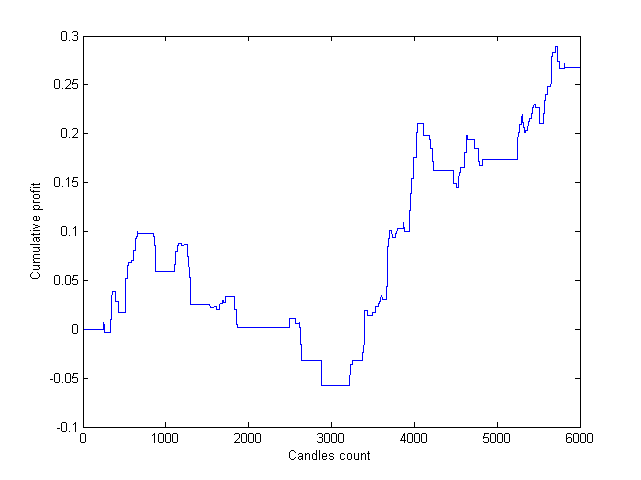
\includegraphics[width = 0.5\textwidth]{pictures/PivotPointsA.png}
\caption{Cumulative profit for sub strategy A}
\label{rys8}
\end{figure}
\FloatBarrier
\noindent The final results of the A sub-strategy:
\begin{itemize}
\item Profit: $0.268$
\item The Calmar ratio: $1.703$
\end{itemize}
\vspace{1em}
\noindent Afterward similar tests of the B sub strategy were run.\\

The confusion matrix presenting the results of the B sub strategy simulations is presented in Table \ref{tab9}.
\begin{table}[ht]
\centering
\caption{Matrix for sub strategy B}
\label{tab9}
\begin{tabular}{|l|l|l|}\hline
&	Actual = profit	& Actual = loss\\ \hline
Prediction = profit & $83$	& $48$ \\ \hline
Prediction = loss &	$2602$ &	$3058$ \\ \hline
\end{tabular}
\end{table}
\FloatBarrier
\noindent The Matthews correlation coefficient is $0.052$.\\
The cumulative profit curve for sub strategy  B is presented in Figure \ref{rys9}.
\begin{figure}[ht]
\centering
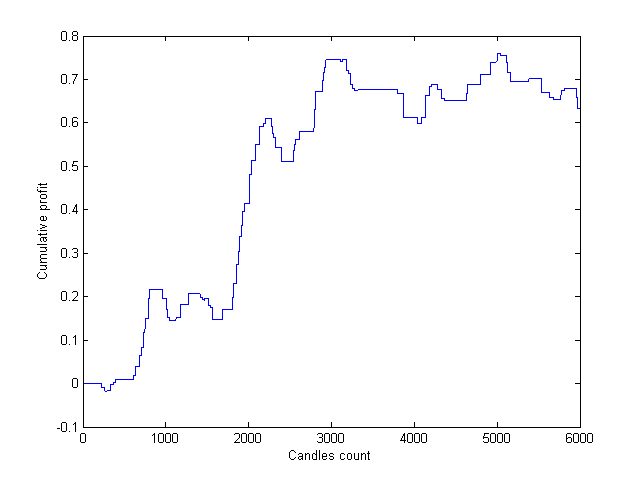
\includegraphics[width = 0.5\textwidth]{pictures/PivotPointsB.png}
\caption{Cumulative profit for sub strategy B}
\label{rys9}
\end{figure}
\FloatBarrier
The final results of the B sub strategy:
\begin{itemize}
\item Profit: $0.633$
\item The Calmar ratio: $4.271$
\end{itemize}
\vspace{1em}
\noindent Afterward similar tests of the C sub-strategy were run.\\

The confusion matrix presenting the results of the C sub strategy simulations looks like in Table \ref{tab10}.
\begin{table}[ht]
\centering
\caption{Matrix for sub strategy C}
\label{tab10}
\begin{tabular}{|l|l|l|}\hline
&	Actual = profit	& Actual = loss\\ \hline
Prediction = profit & $102$	& $53$ \\ \hline
Prediction = loss &	$2743$ &	$2873$ \\ \hline
\end{tabular}
\end{table}
\FloatBarrier
\noindent The Matthews correlation coefficient is $0.055$.\\
The cumulative profit curve looks like in Figure \ref{rys10}.
\begin{figure}[ht]
\centering
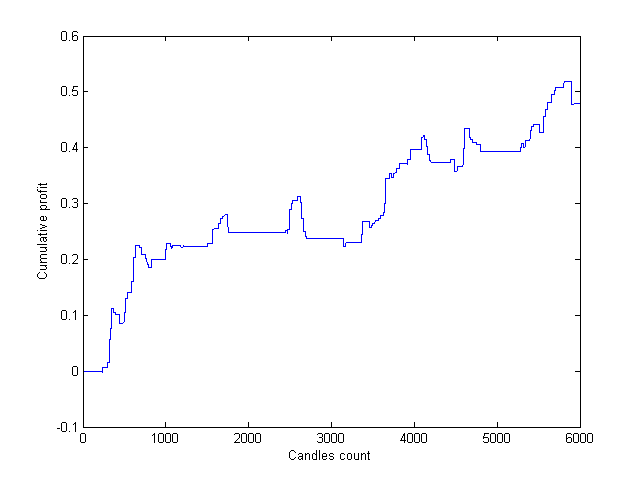
\includegraphics[width = 0.5\textwidth]{pictures/PivotPointsC.png}
\caption{Cumulative profit for sub strategy C}
\label{rys10}
\end{figure}
\FloatBarrier
The final results of the C sub strategy:
\begin{itemize}
\item Profit: $0.478$
\item The Calmar ratio: $5.302$
\end{itemize}
\vspace{1em}
\noindent Afterward similar tests of the D sub-strategy were run.\\
	
The confusion matrix presenting the results of the D sub strategy simulations is presented in Table \ref{tab11}.
\begin{table}[ht]
\centering
\caption{Matrix for sub strategy D}
\label{tab11}
\begin{tabular}{|l|l|l|}\hline
&	Actual = profit	& Actual = loss\\ \hline
Prediction = profit & $79$	& $42$ \\ \hline
Prediction = loss &	$2649$ &	$3063$ \\ \hline
\end{tabular}
\end{table}
\FloatBarrier
\noindent The Matthews correlation coefficient is $0.054$.\\
The cumulative profit curve for sub strategy D is presented in Figure \ref{rys11}.
\begin{figure}[ht]
\centering
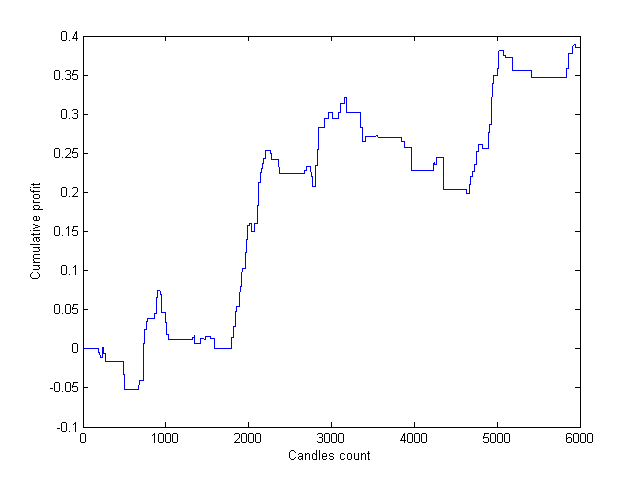
\includegraphics[width = 0.5\textwidth]{pictures/PivotPointsD.png}
\caption{Cumulative profit for sub strategy D}
\label{rys11}
\end{figure}
\FloatBarrier	
The final results of the D sub strategy:
\begin{itemize}
\item Profit: $0.385$
\item The Calmar ratio: $3.129$
\end{itemize}



% % % % % % % % % % % % % % % % % % % % % % % % % %
\section{The summary of the strategies effectiveness with the MCC}
The cumulative profit curve of the summarizing strategy composed of the four sub strategies is presented in Figure \ref{rys12}.
\begin{figure}[ht]
\centering
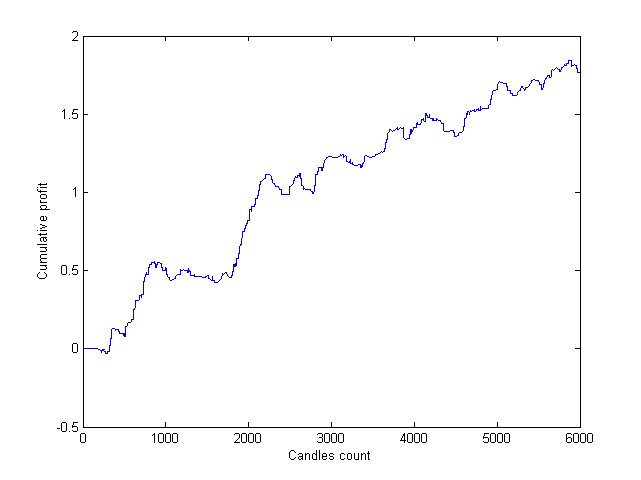
\includegraphics[width = 0.5\textwidth]{pictures/PivotPointsPodsumowanie.png}
\caption{Cumulative profit for sub strategy S}
\label{rys12}
\end{figure}
\FloatBarrier
The confusion matrix presenting the results of the summarizing strategy is presented in Table \ref{tab12}.
\begin{table}[ht]
\centering
\caption{Confusion matrix for summary of all sub strategies}
\label{tab12}
\begin{tabular}{|l|l|l|}\hline
&	Actual = profit	& Actual = loss\\ \hline
Prediction = profit & $366$	& $200$ \\ \hline
Prediction = loss &	$10671$ &	$11941$ \\ \hline
\end{tabular}
\end{table}
\FloatBarrier

\noindent The Matthews correlation coefficient is $0.054$.\\
The final results of the summarizing strategy:
\begin{itemize}
\item Profit: 1.7644
\item The Calmar ratio: 11.991
\end{itemize}
\vspace{1em}
The Table \ref{tab13} presents a summary of the tests results. The authors show also the number of the opened positions and the precision measure, which  is defined as the ratio of the true positives to both true positives and false positives. 
\begin{table}[ht]
\centering
\caption{Optimized values of the parameters for each sub strategy}
\label{tab13}
\begin{tabular}{|l|l|l|l|l|l|}\hline
&	Final profit &	Calmar	& Number of open positions	& Precision & 	MCC \\ \hline
A	& $0.268$	& $1.703$	& $159$	& $0.642$	& $0.054$\\ \hline
B	& $0.633$	& $4.271$	& $131$	& $0.634$	& $0.052$\\ \hline
C	& $0.478$	& $5.302$	& $155$	& $0.658$	& $0.055$\\ \hline
D	& $0.385$	& $3.129$	& $121$	& $0.653$	& $0.054$\\ \hline
S	& $1.764$	& $11.991$	& $566$	& $0.647$	& $0.054$\\ \hline
\end{tabular}
\end{table}
\FloatBarrier
As demonstrated in the table, the MCC values of all the sub strategies and the summarizing one are almost exact. The equality of the values is caused by the similar precision of the sub strategies. Obtained precision measures are supposed to be very high. It may be compared to a 60 percent chance of winning ,,an asymmetrical coin'' toss. It is important to remember that these results were gathered within the training data set. Though, deducing from the gained experience, the authors consider the finding to be remarkable. Since this manner of usage of the MCC is unique, an approximately five-percent value of the MCC was a completely new occurrence. It should be noted that the Calmar ratio achieved values within a significantly wider range. 	
	
% % % % % % % % % % % % % % % % % % % % % % % % % %
\section{Conclusions}

The research of the usefulness of the MCC to evaluate the quality of the strategy does not encourage  to use this indicator. It is clear especially in the last table, that comparable values of MCC values may give different values of Calmar ratio. Generally, however, in confusion matrix lies interesting information especially regarding precision of the strategy. The $TP /( TP + FP )$ ratio resembles the model of asymmetric coins, which  investor  ,,throws''. If the ratio is greater than 50\% than this strategy is promising. The test strategy achieved results far above 60\%. \\

An important result of this work is also paying attention to the low efficiency of the popularized strategies based on the concept of fixed pivot points levels. For authors, it is clear that without the introduction of additional parameters such strategies are useless --- these strategies generate small number of openings and their effectiveness is difficult to statistically prove.


\bibliography{jtacs_tewi}
\bibliographystyle{jtacs}

\end{document}
